Dopo l'introduzione del Boeing 707, uno dei primi jet commerciali ad entrare in servizio, Pan Am richiese un aereo circa due volte e mezzo più grande. Questa esigenza portò allo sviluppo del Boeing 747, che entrò in servizio nel 1970.

Per rispondere a questa esigenza, Boeing progettò un aereo a fusoliera larga con un'apertura alare di 65 metri ed una lunghezza di 70 metri, caratteristiche che gli valsero l'appellativo di "Jumbo Jet".
Il velivolo è spinto da quattro motori turboventola, che gli consentono di raggiungere una velocità massima di crociera di circa 1.040 km/h (Mach 0.85) ed un'autonomia di più di 13.000 km.

Grazie alla sua versatilità, il 747 ebbe un grande successo commerciale: nei 55 anni di produzione, Boeing ne costruì 1.574 esemplari. La maggior parte fu destinata al trasporto passeggeri, ma ne furono prodotte anche versioni cargo e militari.

\begin{figure}[H]
    \centering
    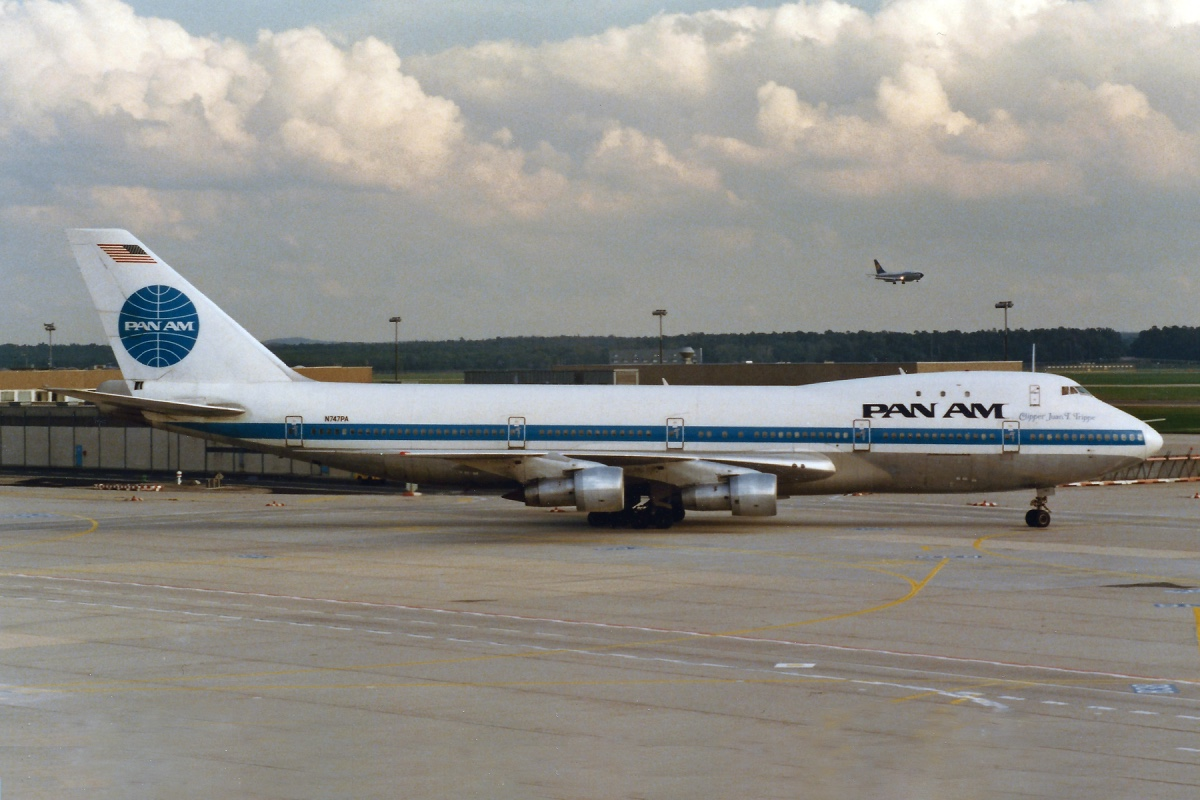
\includegraphics[width=0.65\linewidth]{Immagini/747.jpg}
    \caption{Un Boeing 747 di Pan Am \cite{747-image}}
\end{figure}

\newpage
\section{Sistemi di Riferimento}
Nella descrizione delle forze e delle quantità del velivolo è utile adottare diversi sistemi di riferimento standard utilizzati in aviazione.
Di seguito sono descritti i sistemi di riferimento utilizzati nel corso di questa tesi.

\subsection{Sistema di Riferimento NED}
La Terra sarà considerata un sistema di riferimento inerziale, trascurandone il suo movimento nello spazio in quanto esso è trascurabile rispetto a quello del velivolo.
Inoltre, la curvatura terrestre non verrà considerata: la superficie terrestre sarà approssimata ad un piano infinito.

Il sistema di riferimento $NED$ è un sistema di assi solidale con la Terra e, quindi, anch'esso approssimato come inerziale, con origine posta sulla superficie terrestre. Gli assi sono definiti come segue:
\begin{sitemize}
    \item Asse Down ($\hat{z}_{NED}$) è diretto verso il centro della Terra. Il verso positivo è concorde al verso del vettore di gravità.
    \item Asse North ($\hat{x}_{NED}$) definito dall'intersezione tra il piano orizzontale locale e il piano contenente l'asse di rotazione terrestre. Il verso positivo è orientato verso il nord geografico.
    \item Asse East ($\hat{y}_{NED}$) perpendicolare ai due assi già definiti con il verso positivo nella direzione di rotazione terrestre, in modo da ottenere una terna destrorsa.
\end{sitemize}

\begin{figure}[H]
    \centering
    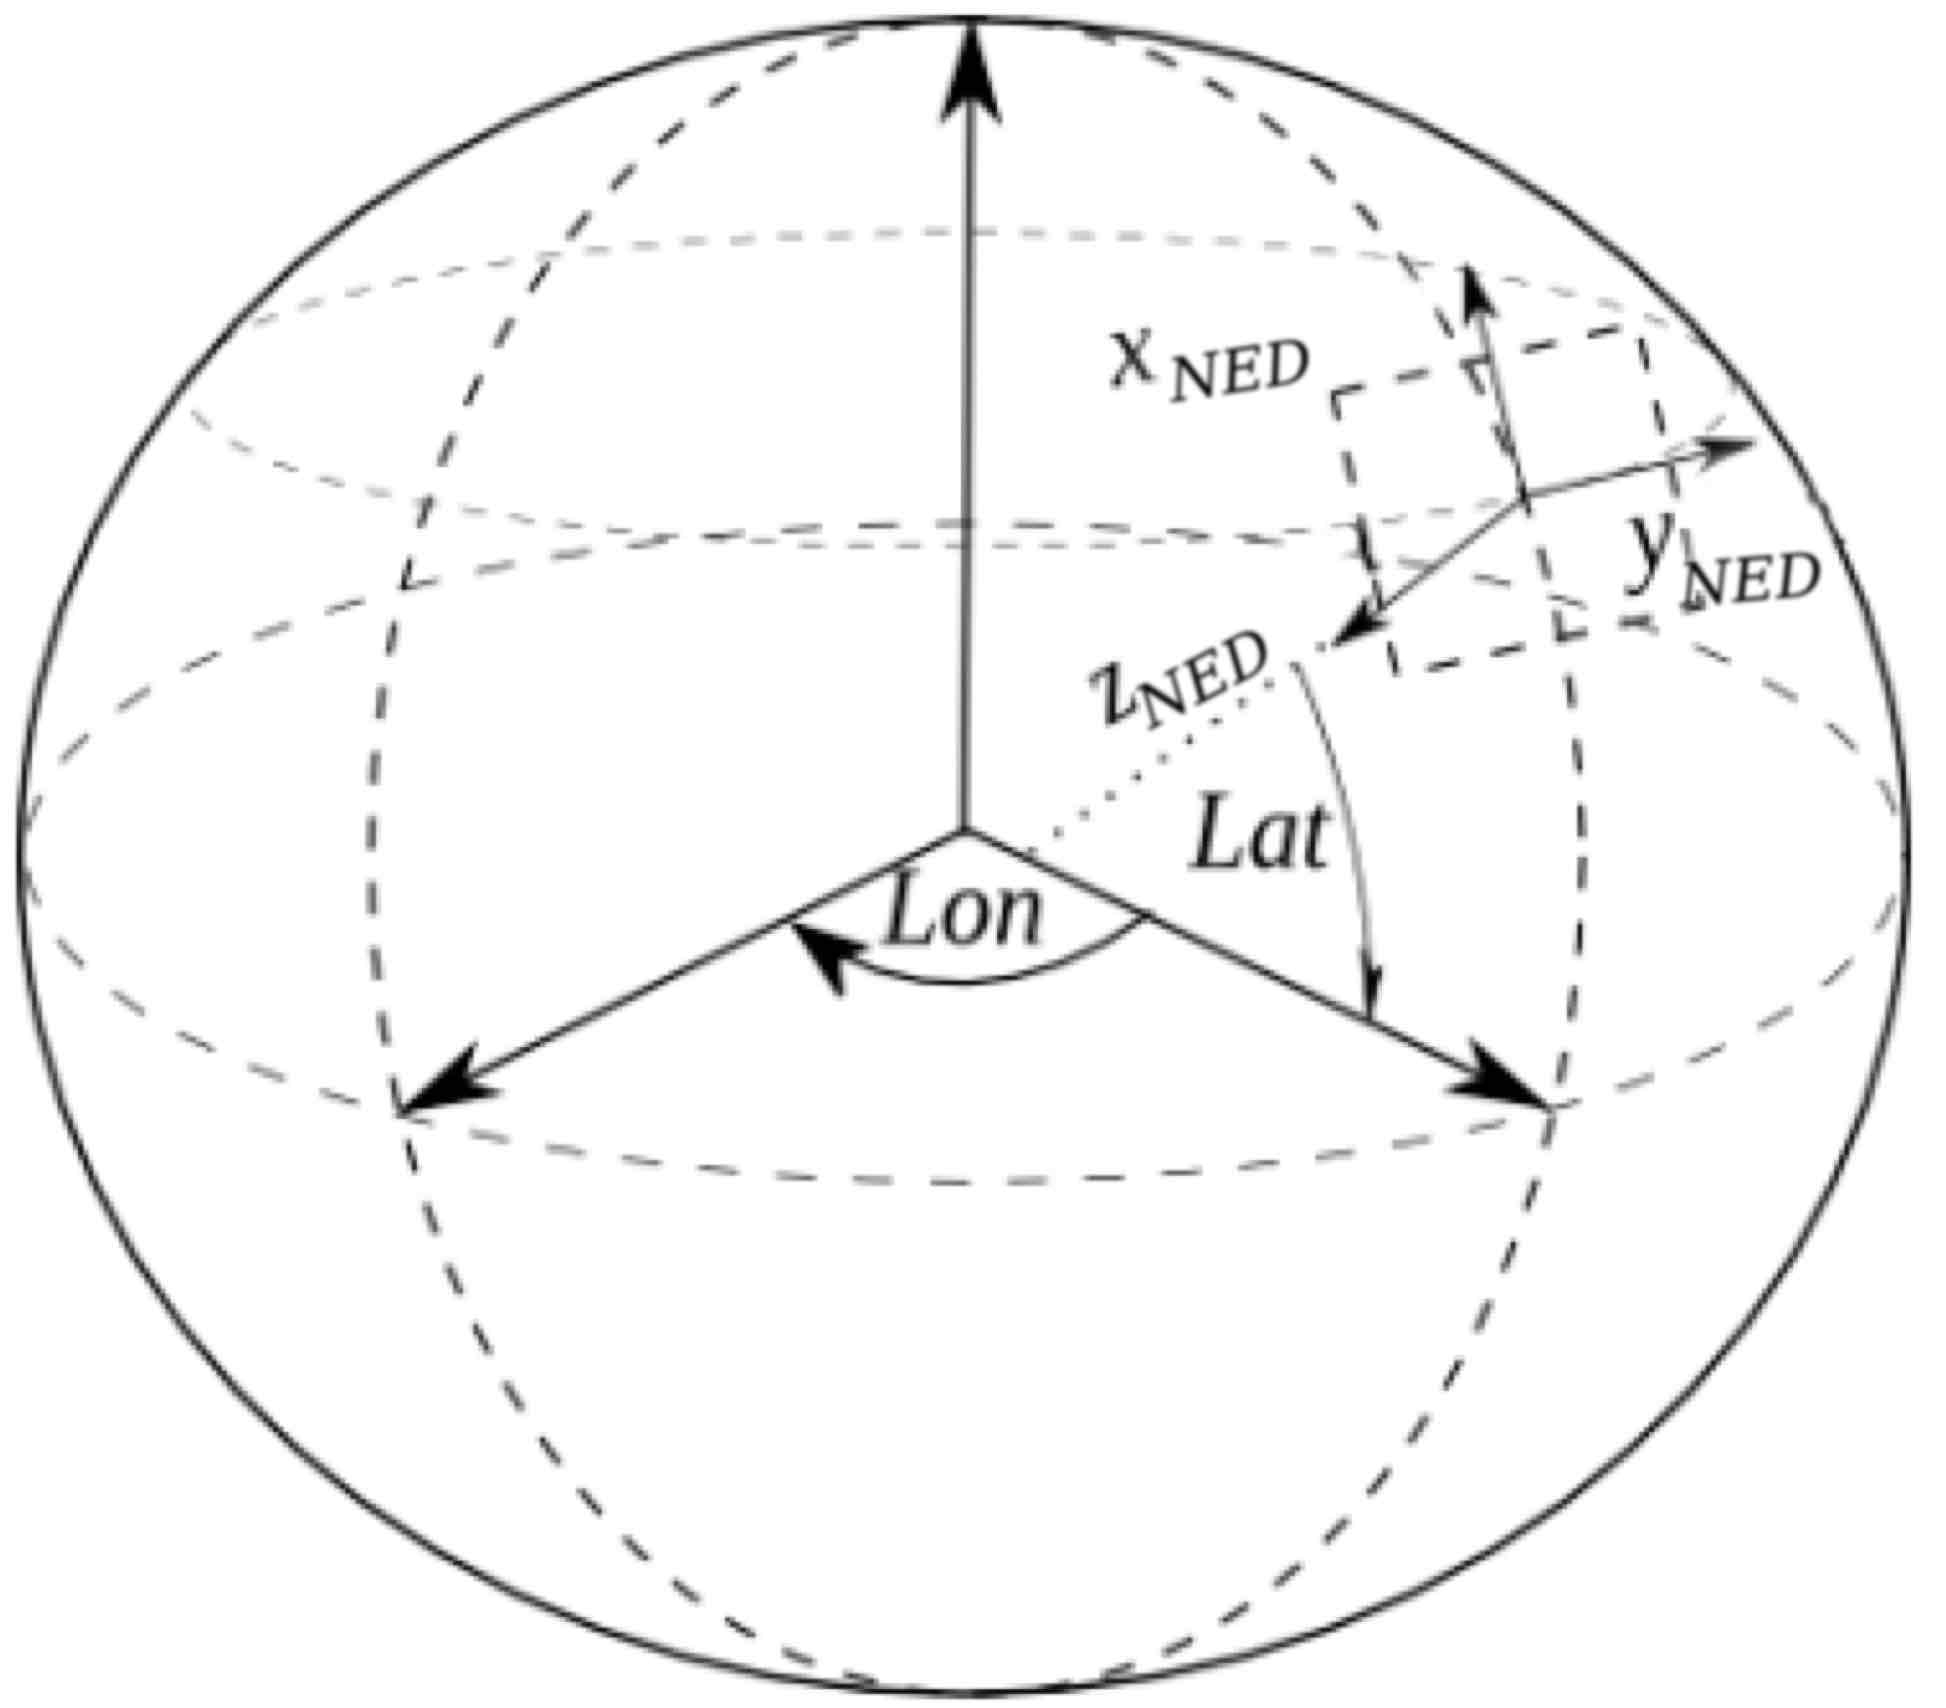
\includegraphics[width=0.4\linewidth]{Immagini/NED.jpg}
    \caption{Sistema di riferimento $NED$ \cite{mscthesis:uav}}
\end{figure}


\subsection{Sistema Assi Corpo FRD}

Il sistema assi corpo, o Front-Right-Down ($FRD$) ha origine nel centro di massa del velivolo. Gli assi sono definiti nel seguente modo:

\begin{sitemize}
    \item Asse ($\hat{x}_{FRD}$) è parallelo alla linea di riferimento della fusoliera ed è diretto nella direzione in cui è rivolto il pilota
    \item Asse ($\hat{y}_{FRD}$) passa attraverso le punte delle ali, con verso positivo verso la destra del velivolo.
    \item Asse ($\hat{z}_{FRD}$) è diretto verso il basso, perpendicolare agli altri due assi.
\end{sitemize}

\begin{figure}[H]
    \centering
    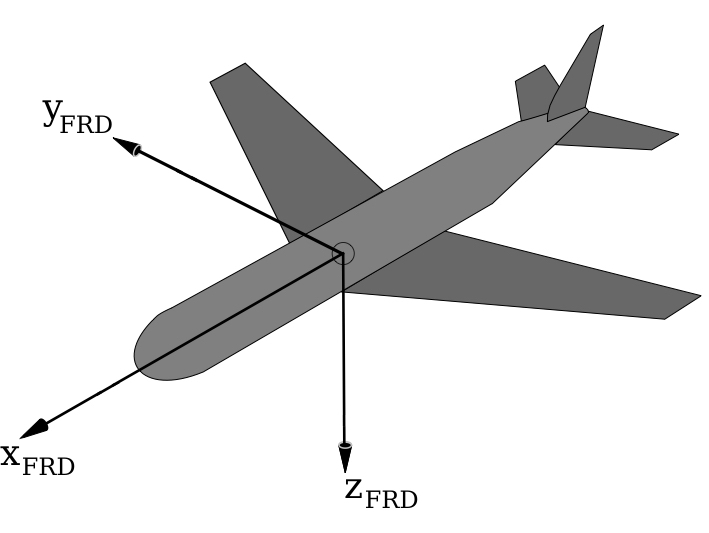
\includegraphics[width=0.42\linewidth]{Immagini/FRD.jpg}
    \caption{Sistema di riferimento $FRD$ \cite{wiki:FRD}}
\end{figure}

\subsection{Sistema Assi di Stabilità}
Solitamente il velivolo presenta un certo angolo di incidenza $\alpha$ rispetto al flusso d'aria durante il volo.
Viene definito quindi il sistema assi di stabilità, i cui versori sono detti $\hat{x}_{S}$, $\hat{y}_{S}$, $\hat{z}_{S}$, ottenuto effettuando una rotazione del sistema di riferimento $FRD$ di un angolo $\alpha$ attorno all'asse $\hat{y}_{FRD}$.

\begin{figure}[H]
    \centering
    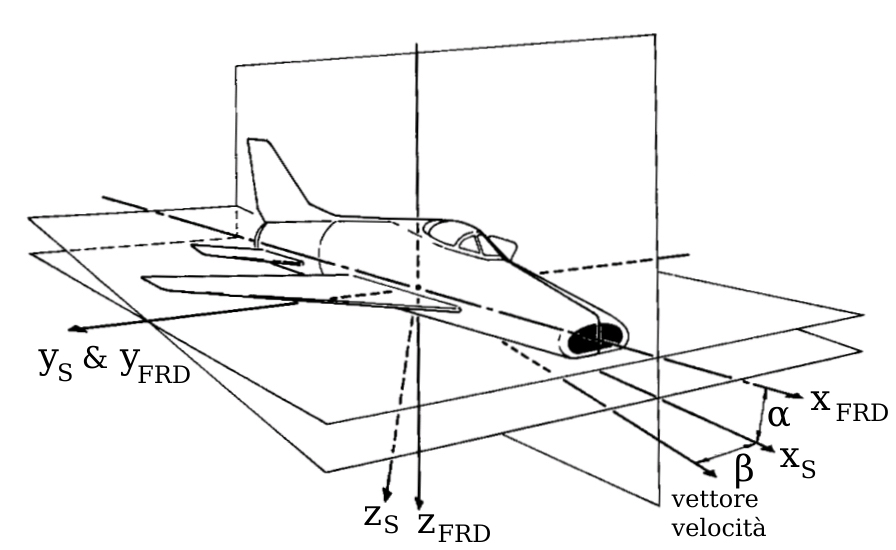
\includegraphics[width=0.5\linewidth]{Immagini/stability.jpg}
    \caption{Sistema di riferimento Assi di Stabilità \cite{mscthesis:jetfighter}}
\end{figure}

\subsection{Sistema Assi Vento}
Un aereo può volare anche con un certo angolo di derapata $\beta$ rispetto al flusso d'aria.
Viene definito quindi il sistema assi vento, i cui versori sono detti $\hat{x}_{W}$, $\hat{y}_{W}$, $\hat{z}_{W}$, ottenuto effettuando una rotazione del sistema assi di stabilità di un angolo $\beta$ attorno all'asse $\hat{z}_{S}$.

\begin{note}
    Si nota che non è necessaria alcuna rotazione attorno all'asse $\hat{x}_{W}$ per allinearlo al vettore velocità, quindi nella trasformazione al sistema assi vento quell'angolo di rotazione rimane 0.
\end{note}
